\section{Résultats}
\subsection{Procédure d'évaluation}
\noindent
Afin d'évaluer les performances de notre structure de données en matière de ressources mémoires ainsi qu'en vitesse de navigation, nous avons implémenté la totalité des procédures décrites dans ce rapport et effectué une comparaison avec d'autres structures de données existantes.\\
Tout le code est implémenté en C\texttt{++} natif, sans l'aide d'aucune bibliothèque extérieure. Le code source est compilé avec g\texttt{++} sous Elementary OS. Tous les algorithmes ont été exécutés sur une machine avec un processeur i5-5300U et 16Go de RAM. L'ensemble du code est open-source et disponible sur github : \url{https://github.com/beaupletga/3D-Mesh-Compression}.\\
Pour effectuer nos tests, nous avons choisi une dizaine de maillages avec des formes, des tailles, et des tétraédrisations différentes (Fig. \ref{fig:exemples_maillages}). Les boules ont été générées avec CGAL \cite{CGAL} en utilisant le module de génération de sphères implicites. Les autres tétraédrisations ont été pris le site \textit{Aim@Shape}. Nous ne présentons les résultats de nos algorithmes que sur 8 de ces maillages.
\begin{figure}[th]
\centering
\begin{subfigure}{.24\textwidth}
  \centering
  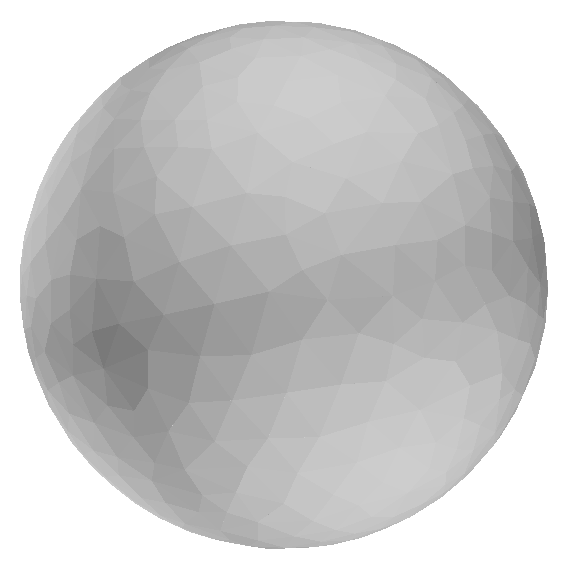
\includegraphics[scale=0.12]{Images/ball}
%  \caption{figure}{Tétraèdrisation d'une boule}
%  \label{fig:ball}
\end{subfigure}%
\begin{subfigure}{.24\textwidth}
  \centering
  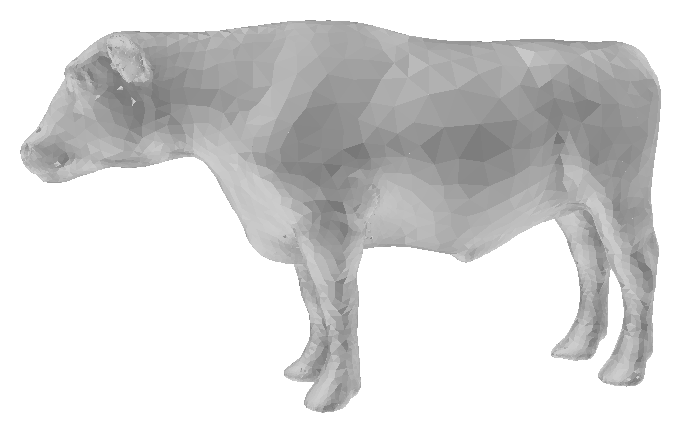
\includegraphics[scale=0.12]{Images/cow}
%  \caption{figure}{Tétraèdrisation d'une vache}
%  \label{fig:cow}
\end{subfigure}
\begin{subfigure}{.24\textwidth}
  \centering
  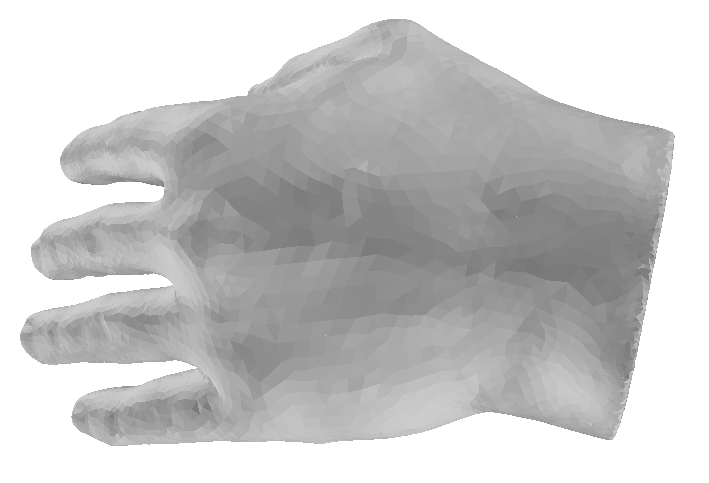
\includegraphics[scale=0.12]{Images/hand}
%  \caption{figure}{Tétraèdrisation d'une main}
%  \label{fig:hand}
\end{subfigure}%
\begin{subfigure}{.24\textwidth}
  \centering
  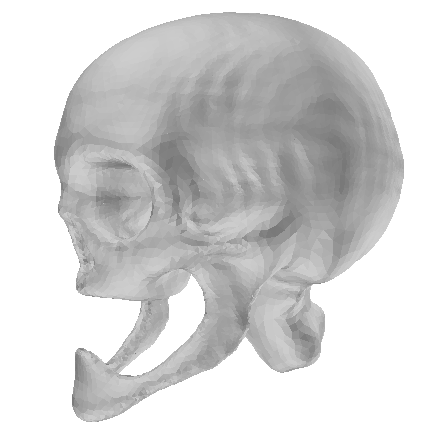
\includegraphics[scale=0.14]{Images/skull}
%  \caption{figure}{Tétraèdrisation d'un crane}
%  \label{fig:skull}
\end{subfigure}
\caption{Exemples de maillages tétraédriques utilisés pour évaluer notre structure de données.}
\label{fig:exemples_maillages}
\end{figure}

\begin{table}[H]
\centering
\footnotesize
\begin{tabular}{|c | c | c | c | c| c | c |}
\hline
Nom de la & Nombre de & Nombre& Nombre de & Part de tétraèdres & Nombre de & Nombre d'arêtes\\
structure&sommets&d'arêtes &tétraèdres&sur les bords&tétraèdres par sommet & par sommet\\
\hline
Boule (B1) & 1k & 5k & 3k & 0.45 & 13.52 & 10.32 \\
Boule (B2)& 15k & 101k & 83k & 0.07 & 22.15 & 13.45\\
Boule (B3)& 378k & 2M & 2.2M & 0.05 & 23.70 & 13.98 \\
Boule (B4)& 1.3M & 9.5M & 8.1M & 0.01 & 24 & 14 \\
Boule (B5)& 1.7M & 12.1M & 10.3 & 0.01  & 24.03  & 14.01  \\
Vache (V1)& 30k & 182k & 134k & 0.24 & 17.48 & 11.82 \\
Main (M1)& 28k & 169k & 125k & 0.24 & 17.38 & 11.74\\
Crane (C1)& 37k & 217k & 156k & 0.30 & 16.51 & 11.52 \\ 
\hline  
\end{tabular}
\caption{Caractéristiques des maillages tétraédriques utilisés pour évaluer notre structure}
\label{tab:caract_maillages}
\end{table}

\subsection{Appariement des tétraèdres en diamants}
\noindent
On peut évaluer l'appareillage des tétraèdres en diamants en regardant la part des tétraèdres dans des diamants ou en calculant le nombre de références par tétraèdre (rpt). On calcule ce dernier de cette manière :\\
\begin{equation}
\text{rpt} = \frac{2\cdot T_D+4\cdot T_i}{|T|}
\end{equation}
\begin{table}[H]
\centering
\footnotesize
\begin{tabular}{|c | c | c | c| c | c | c |}
\hline
& \multicolumn{3}{|c|}{Parcours en largeur}& \multicolumn{3}{|c|}{Degré de l'arête}\\
\hline
Nom de la & Part des tétraèdres & RPT & Temps (s) & Part des tétraèdres & RPT & Temps (s)\\
structure&dans des diamants (\%)&&&dans des diamants (\%)&&\\
\hline
B1 & 76 & 2.69 & 0.03 & 81 & 2.36 & 0.47 \\
B2 &  80 & 2.39 & 1.02 & 85 & 2.29 & 497 \\
B3 & 81& 2.37 & 39.79 &  &  &\\
B4 & 82& 2.35 & 150 &  &  &\\
B5 & 82 & 2.35 & 172 &  &  &\\
V1 & 77& 2.44 & 1.56 & 81& 2.36 & 922\\
M1 & 77& 2.44 & 1.26 & 83 & 2.34 & 794\\
C1 & 77& 2.44 & 1.48 & 80 & 2.38 & 1262\\
\hline  
\end{tabular}
\caption{Résultats des algorithmes d'appareillage des tétraèdres en diamants. Le deuxième algorithme ayant des temps de calcul assez importants, certains maillages n'ont pas pu être considérés.}
\label{tab:results_performances}
\end{table}

\begin{figure}[H]
\begin{center}
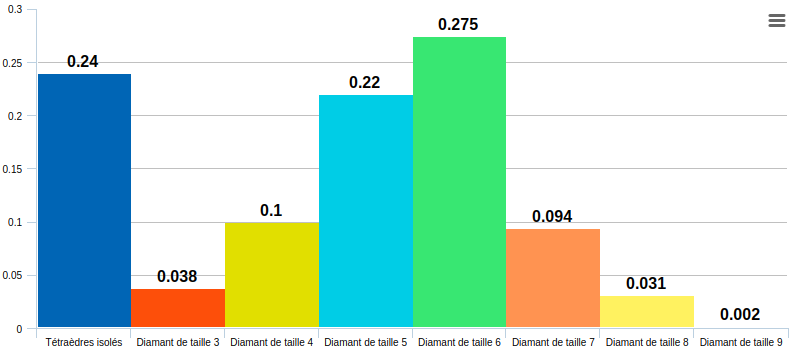
\includegraphics[scale=0.36]{Images/histograme}
\caption{Histogramme de la part de tétraèdres parmi les tétraèdres isolés et diamants en utilisant le parcours en largeur}
\label{fig:histogramme}
\end{center}
\end{figure}
\begin{figure}[H]
\centering
\pgfplotsset{width=15cm,height=5.5cm}
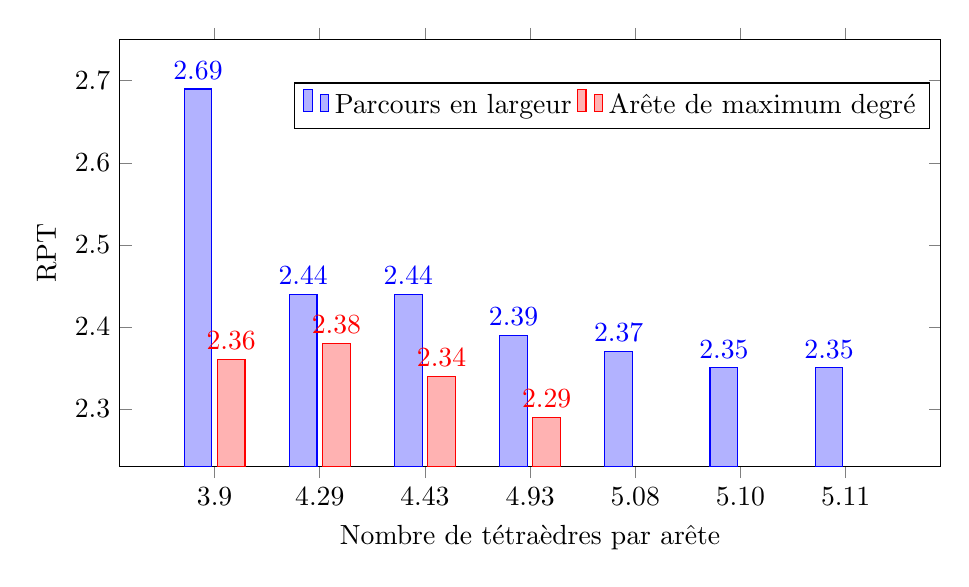
\begin{tikzpicture}
\begin{axis}[
    ybar,
    enlargelimits=0.15,
    legend style={at={(0.6,0.9)},
      anchor=north,legend columns=-1},
    ylabel={RPT},
    xlabel={Nombre de tétraèdres par arête},
    symbolic x coords={3.9,4.29,4.43,4.93,5.08,5.10,5.11},
    xtick=data,
    nodes near coords,
    nodes near coords align={vertical},
    ]
\addplot coordinates {(3.9,2.69)(4.29,2.44)(4.43,2.44)(4.93,2.39)(5.08,2.37)(5.10,2.35)(5.11,2.35) };
\addplot coordinates {(3.9,2.36)(4.29,2.38)(4.43,2.34)(4.93,2.29)(5.08,)(5.10,)(5.11,) };
\legend{Parcours en largeur,Arête de maximum degré}
\end{axis}
\end{tikzpicture}
\caption{Nombre de références par tétraèdre (rpt) en fonction du nombre de tétraèdres par arête}
\label{fig:graphique}
\end{figure}

\vspace{0.1cm}
\noindent
On note sur la Fig. \ref{fig:graphique} qu'il semble avoir un lien entre le nombre de tétraèdres par arête et les performances de nos algorithmes de création de diamants. Ce comportement ne semble pas étonnant étant donné que plus le nombre de tétraèdres par arête est important, plus les diamants peuvent contenir un nombre important de tétraèdres. Compte tenu des résultats de Tab. \ref{tab:results_performances}, nous avons choisi d'utiliser le parcours en largeur pour appareiller les tétraèdres en diamants. Le parcours en largeur est rapide et permet d'associer en moyenne 76\% des tétraèdres en diamants. Néanmoins, notre algorithme pourrait probablement être amélioré en étant exécuté en parallèle ou en choisissant plus spécifiquement un tétraèdre de départ (Fig. \ref{fig:bfs_starting}). On remarque que 50\% des tétraèdres sont dans des diamants possédant 5 ou 6 tétraèdres (Fig. \ref{fig:histogramme}).

\subsection{Ancrage des sommets}
\begin{table}[H]
\footnotesize
\centering
\begin{tabular}{|c | c | c | c |}
\hline
Nom de la & Part de sommets non associés & Part de tétraèdres dans  & Part de tétraèdres dans \\
structure&avec des diamants  & des diamants avant & des diamants après \\
& ou tétraèdres isolés (\%) & choix des ancres (\%)& choix des ancres (\%)\\
\hline
B1 & 6 & 76& 65 \\
B2 & 0.08& 80 & 80 \\
B3 & 0.03& 82 & 82\\
B4 & 0.01 & 82 & 82\\
B5 & 0.02 & 82 & 82\\
V1 & 0.8  & 77 & 76 \\
M1 & 0.7 & 77& 76\\
C1 & 0.8 & 77 & 76 \\
\hline  
\end{tabular}
\caption{Résultats de l'ancrage des sommets aux diamant/tétraèdres isolés en utlisant un algorithme glouton affectant en priorité les sommets adjacents à peu de diamants/tétraèdres isolés}
\label{tab:results_ancres}
\end{table}
\noindent
On remarque sur le Tab. \ref{tab:results_ancres} qu'en appliquant l'algorithme glouton afin d'appareiller sommets et diamants/tétraèdres isolés, une part minime des sommets demeure non ancrée (1ère colonne). Par ailleurs, on note que la destruction de certains diamants pour associer des sommets à des tétraèdres n'a que peu d'incidence sur la part de sommets ancrés tant que le nombre de sommets est important (2ème et 3ème colonnes).

\newpage
\subsection{Les requêtes}
\noindent
Pour évaluer le temps nécessaire pour répondre à une requête, nous évaluons celle-ci après 10 000 essais aléatoires. Les temps sont obtenus en utilisant l'optimisation '-O3' de C\texttt{++}.
\begin{savenotes}
\begin{table}[h]
\footnotesize
\centering
\begin{tabular}{| c | c | c| c |c |c|}
\hline
Nom de la & Accès au& Accès au & Degré d'un & Parcours en & Parcours en\\
structure &$i$-ème tétraèdre (s)& $i$-ème diamant (s) &sommet (s)&largeur (s) & largeur normalisé\footnote{Par rapport au nombre de tétraèdres} (s/tétraèdre)\\
\hline
B1  & 1e-5 & 5e-6 & 1.9e-5 & 6e-4& 1.67e-7 \\
B2  &  4.1e-4 & 1.6e-4 & 1.2e-4 & 0.01& 1.19e-7\\
B3 & 0.011 & 0.0042 & 0.002 & 0.8&3.56e-7\\
B4 & 0.01 & 0.01 & 0.01 & 4.6&5.6e-7\\
B5 & 0.04 & 0.01 & 0.01 & 4.46& 4.3e-7 \\
%V1 & & & & \\
M1  & 6.4e-4 & 2.6e-4 & 2.2e-4 & 0.02&1.59e-7\\
C1  & 8.1e-4 & 3.4e-4 & 2.8e-4 & 0.02&1.28e-7\\
\hline  
\end{tabular}
\label{table:results_time}
\caption{Temps requis (s) pour répondre aux requêtes sur plusieurs maillages}
\end{table}
\end{savenotes}
\noindent

%Temps moyen structure de données non compacte (4 references tétra)
%1.8e-3 7.8e-4 1.9e-4 0.36
%2.5e-3 9.9e-4 5.2e-4 0.17
%
\begin{figure}[H]
\centering
\pgfplotsset{width=12cm,height=7cm}
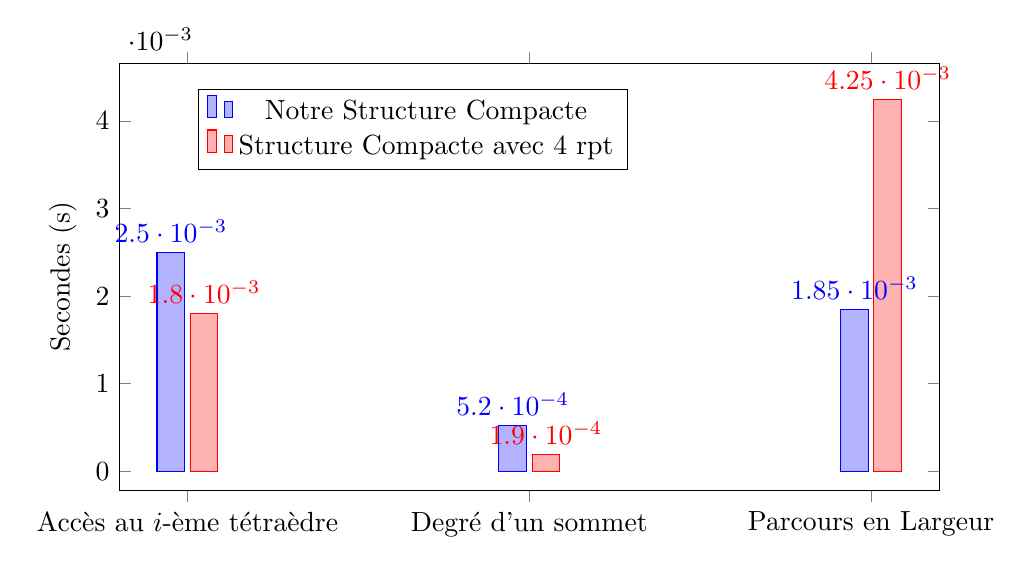
\begin{tikzpicture}
\begin{axis}[
    ybar,
    enlargelimits=0.1,
%    legend style={anchor=east},
    legend style={at={(0.62,0.94)}},
%    anchor=north,legend columns=-1,cells={align=left}},
    ylabel={Secondes (s)},
%    xlabel={Nombre de tétraèdres par arête},
    symbolic x coords={Accès au $i$-ème tétraèdre,Degré d'un sommet,Parcours en Largeur},
    xtick=data,
    nodes near coords,
    nodes near coords align={vertical},
    ]
\addplot coordinates {(Accès au $i$-ème tétraèdre,2.5e-3)(Degré d'un sommet,5.2e-4)(Parcours en Largeur,1.85e-3)};
\addplot coordinates {(Accès au $i$-ème tétraèdre,1.8e-3)(Degré d'un sommet,1.9e-4)(Parcours en Largeur,4.25e-3)};
%\addplot coordinates {(Degré d'un sommet,1e-3)(Parcours en Largeur,2.92e-3)};
%\addplot coordinates {(3.9,2.36)(4.29,2.38)(4.43,2.34)(4.93,2.29)(5.08,)(5.10,)(5.11,) };
\legend{Notre Structure Compacte,Structure Compacte avec 4 rpt,Structure avec Pointeurs}
\end{axis}
\end{tikzpicture}
\caption{Comparaison des temps moyens (s) requis pour répondre aux requêtes et effectuer la navigation dans le maillage. Notre structure de données compacte (en bleue) est comparée à une  structure de données compacte utilisant 4 rpt (i.e SOT). Le temps pour le parcours en largeur est normalisé pour 100K tétraèdres.}
\label{fig:temps_moyen}
\end{figure}
\noindent
Sur Fig. \ref{fig:temps_moyen}, on constate que les temps de calcul de notre structure de données compacte sont moins bons pour l'accès au $i$-ème tétraèdre et le calcul du degré d'un sommet\footnote{Nous n'affichons pas le temps d'accès au $i$-ème diamant car la structure de données compacte à 4 rpt ne réunit pas les tétraèdres en diamants}. Etant donné que dans notre structure de données, le $i$-ème tétraèdre est plus proche du début du tableau que dans la structure à 4 rpt, le résultat devrait être l'inverse. De la même manière, pour le calcul du degré d'un sommet, sachant que les tétraèdres sont regroupés en diamants dans notre structure, le degré devrait être plus rapidement calculé. Nous expliquons ces deux écarts par les comparaisons effectuées dans les requêtes. En effet, lorsque nous voulons calculer le degré d'un sommet, si le sommet est adjacent à un tétraèdre isolé, alors il suffit de localiser la face du tétraèdre isolé non adjacente au sommet puis de naviguer au sein des trois autres faces. En revanche, lorsque notre sommet est adjacent à un diamant, davantage de comparaisons sont nécessaires afin de connaître les faces adjacentes au sommet. Cette supposition est confirmée en analysant les temps requis pour le parcours en largeur du graphe. Lorsque nous effectuons un parcours en largeur du graphe, aucune comparaison (utilisant les permutations des sommets) n'est nécessaire, il suffit seulement d'accéder au diamant/tétraèdres adjacents. Sachant que les tétraèdres sont regroupés en diamants dans notre structure, en accédant à un diamant $D_i$, on accède directement au $|D_i|$ tétraèdres le composant, gagnant un temps non négligeable. 
%Par ailleurs, nous avons choisi de d'ajouter à la comparaison une structure compacte (avec un regroupement en diamants) utilisant les pointeurs (et non un tableau d'entiers). On s'aper\c oit
\subsection{Taille mémoire}
\begin{figure}[H]
\centering
\resizebox{0.65\textwidth} {!}{
\pgfplotsset{width=13cm,height=7cm}
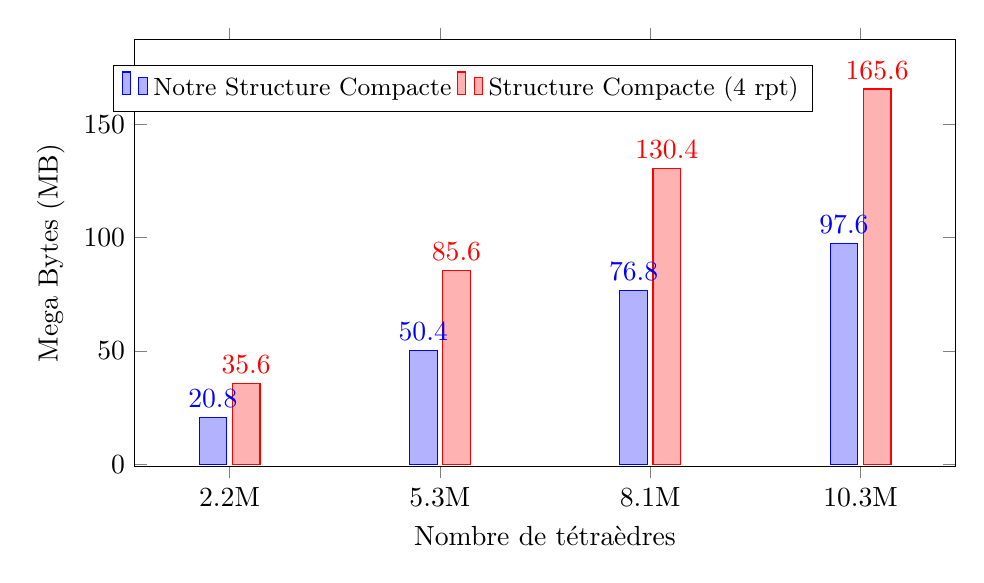
\begin{tikzpicture}
\begin{axis}[
    ybar,
%    ymode = log,
    enlargelimits=0.15,
    legend style={at={(0.4,0.94)},
      anchor=north,legend columns=-1,font=\fontsize{9}{9}\selectfont},
    ylabel={Mega Bytes (MB)},
    xlabel={Nombre de tétraèdres},
    symbolic x coords={2.2M,5.3M,8.1M,10.3M},
    xtick=data,
    nodes near coords,
    nodes near coords align={vertical},
    ]
%\addplot coordinates {(3k,9234)(83k,199262)(125k,307500)(156k,384156)(2.2M,5291508)(8.1M,19212158)(10.3M,24407986)};
%\addplot coordinates {(3k,14332)(83k,333648)(125k,500508)(156k,624540)(2.2M,8.97e6)(8.1M,3.26e7)(10.3M,4.14e7)};
\addplot coordinates {(2.2M,20.8)(5.3M,50.4)(8.1M,76.8)(10.3M,97.6)};
\addplot coordinates {(2.2M,35.6)(5.3M,85.6)(8.1M,130.4)(10.3M,165.6)};
\legend{Notre Structure Compacte,Structure Compacte (4 rpt)}
\end{axis}
\end{tikzpicture}
}
\caption{Comparaison de la taille mémoire (en Mega Bytes) de notre structure de données compacte (en bleue) et de la même structure de données sans regroupement des tétraèdres en diamants (i.e SOT)}
\label{fig:taille_memoire}
\end{figure}
\noindent
La Fig. \ref{fig:taille_memoire} compare l'évolution de la place mémoire en fonction du nombre de tétraèdres par maillage pour notre structure de données et une structure de données utilisant 4 références par tétraèdres. Cette dernière structure de données est équivalente à SOT, seulement son interface de navigation utilise les faces plutôt que les coins pour accéder aux éléments du maillage. Sur le plus gros maillage, notre structure de données permet d'économiser 68MB de place mémoire.

%
%temps pour la structure non compacte
%B1 1.31e-5 5.3e-6 2.7e-5 9.1e-4
%B2 2e-4 & 1e-4 7.1e-5 0.03
%B3 8.1e-3 3e-3 7e-4 1.8
%B4 
%M1 4.9e-4 1.9e-4 8.6e-5 0.04
%C1 6.4e-4 2.7e-4 1.1e-4 0.06

